
\section{Solution 1}
\label{sec:auswertung}


\section{Solution 2}
\label{sec:auswertung}
    \begin{itemize}
        \item[a)]
            In the second exercise we were asked to solve the Lorentz equations 
            \begin{align*}
                \dot{X} = & -\sigma X + \sigma Y \\
     ̇           \dot{Y} = & -XZ + rX - Y \\
     ̇           \dot{Z} = & XY - bZ
            \end{align*}
            with the fourth order Runge-Kutta scheme.
            The implementation can be found in file "2.cpp".
            The parameters $r, \sigma$ and $b$ were given as:
            \begin{align*}
                r = & 20 \,\text{or}\, 28\\
                \sigma = & 10 \\
                b = & 8/3
            \end{align*}
            In the following plots one can clearly see that a change in the starting parameter such as $r$ results in a different behaviour.
            One gives a stable orbit around an attractor, the other falls into the attractor.
            Other parameters show even different behaviour.
            However, the starting position does not influecs the trajectory.
        \item[b)]
            After the implementation we were asked to visualize our solution.
            This should be done in three ways
            \begin{itemize}
                \item[1.]
                    First as a projection of the trajectory on the xy-plane.
                    \FloatBarrier
                    \begin{figure}
                        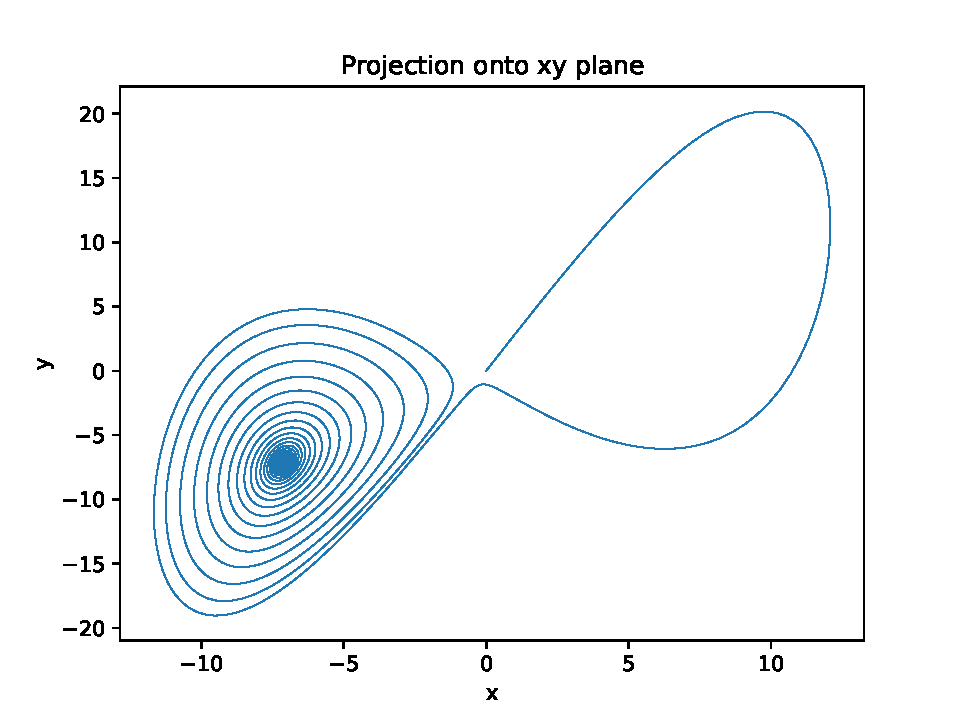
\includegraphics[width=\textwidth]{images/Lorentz_r_20_projection.pdf}
                        \caption{The projection of the trajectory onto the xy-plane with the starting parameter $r=20$.}
                    \end{figure}
                    \begin{figure}
                        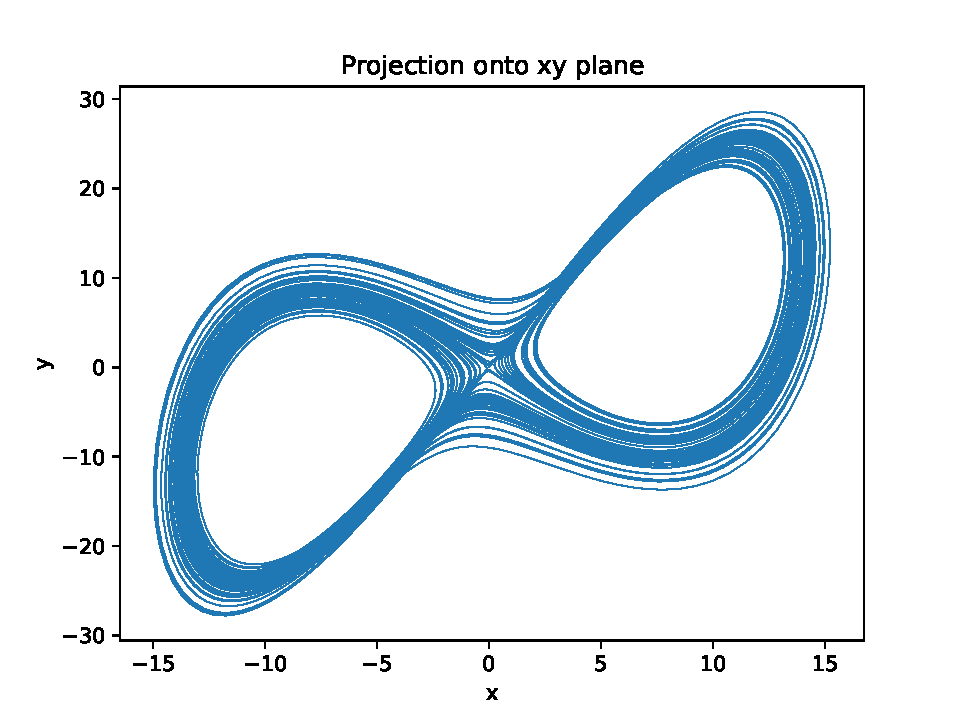
\includegraphics[width=\textwidth]{images/Lorentz_r_28_projection.pdf}
                        \caption{The projection of the trajectory onto the xy-plane with the starting parameter $r=28$.}
                    \end{figure}
                    \FloatBarrier
                \item[2.]
                    As a Poincare slice at $Z=20$ with the condition that $\dot{Z} < 0$.
                    We tested for this condition by subtracting the $\vec{f}(t_i)$ with $\vec{f}(t_{i+1})$. 
                    If the result is basically a linear interpolation between point $\vec{f}(t_i)$ and $\vec{f}(t_{i+1})$.
                    We then plotted all points that forfill the two conditions onto a xy-plane.
                    \FloatBarrier
                    \begin{figure}
                        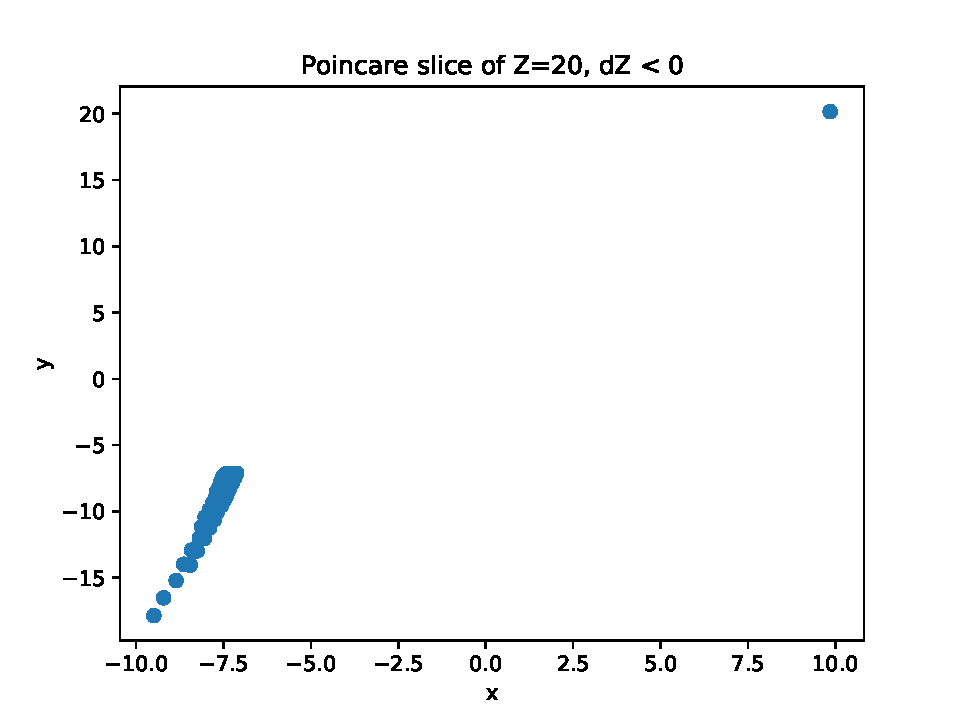
\includegraphics[width=\textwidth]{images/Lorentz_r_20_slice.pdf}
                        \caption{The Poincare slice of the trajectory onto the xy-plane with the starting parameter $r=20$.}
                    \end{figure}
                    \begin{figure}
                        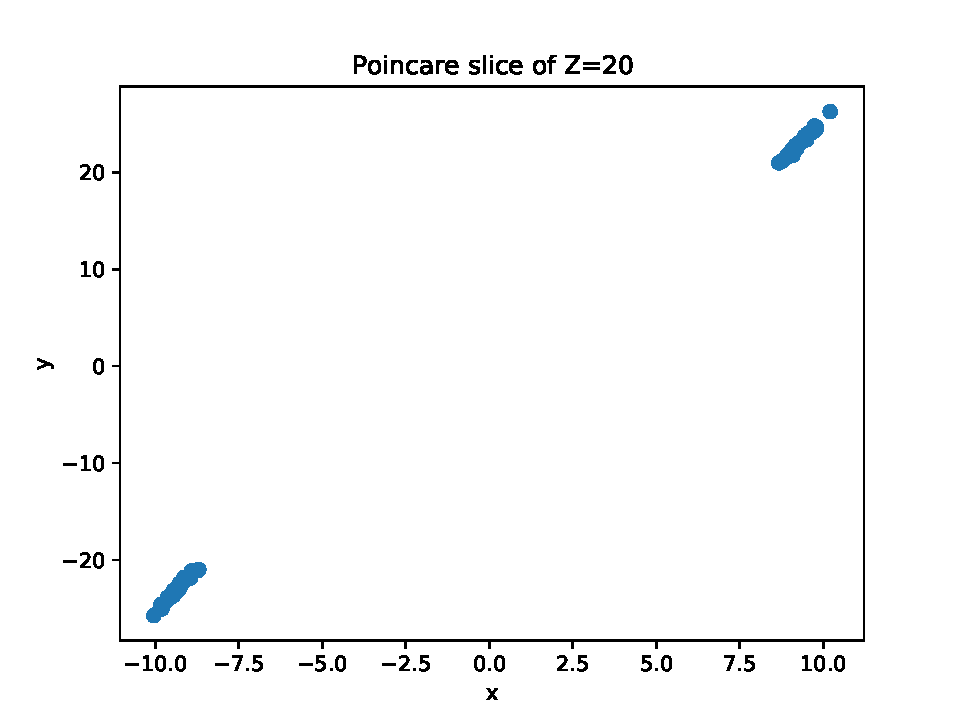
\includegraphics[width=\textwidth]{images/Lorentz_r_28_slice.pdf}
                        \caption{The Poincare slice of the trajectory onto the xy-plane with the starting parameter $r=28$.}
                    \end{figure}
                    \FloatBarrier
                \item[3.]
                    For the last part we plotted the whole xyz-trajectory onto a 3d-plot.
                    \FloatBarrier
                    \begin{figure}
                        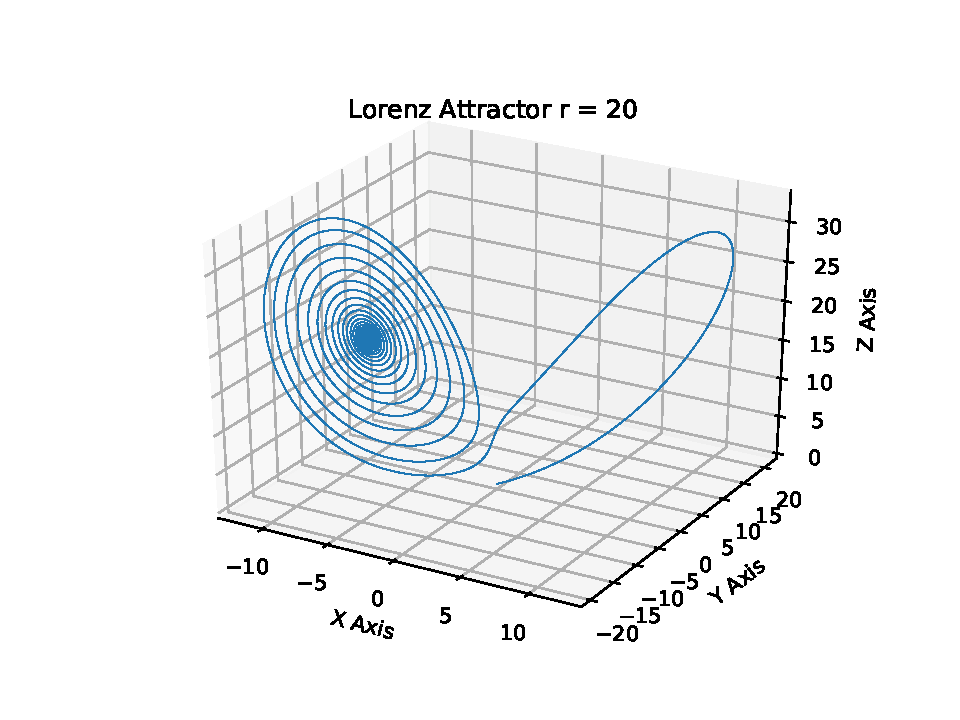
\includegraphics[width=\textwidth]{images/Lorentz_r_20_3d.pdf}
                        \caption{The 3d-Plot of the trajectory with the starting parameter $r=20$.}
                    \end{figure}
                    \begin{figure}
                        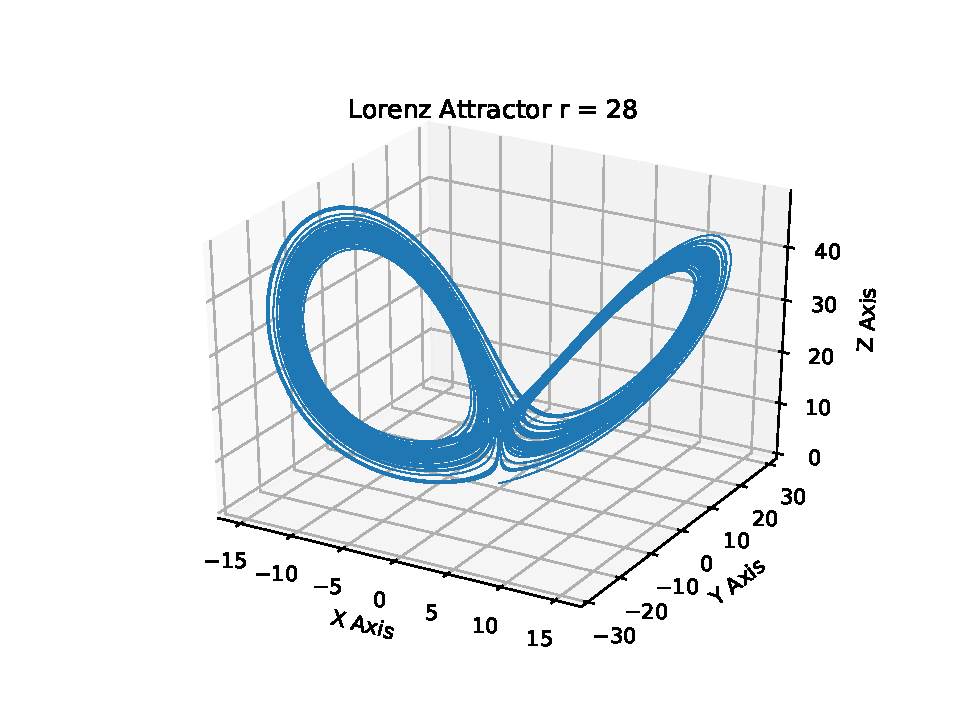
\includegraphics[width=\textwidth]{images/Lorentz_r_28_3d.pdf}
                        \caption{The 3d-Plot of the trajectory with the starting parameter $r=28$.}
                    \end{figure}
            \end{itemize}
\end{itemize}              